\documentclass[main.tex]{subfiles}
\begin{document}

\chapter{The Linear Model}\label{ch:dogrusal}

Linear regression is where all the tools of statistical theory come together: estimation (least squares\index{least squares ls@least squares (LS)}, Gauss--Markov\index{gauss markov theorem@Gauss--Markov theorem}), distribution theory (the multivariate normal\index{multivariate normal distribution@multivariate normal distribution} and quadratic forms), hypothesis testing ($t$ and $F$ tests, likelihood ratio) and interval estimation (confidence and prediction intervals\index{prediction interval@prediction interval}). In this chapter we study the geometry of the linear model\index{linear model@linear model}, the finite-sample and asymptotic properties of the least squares estimator, and exact inference under the assumption of normal errors. The multivariate normal results of Chapter~\ref{ch:ortak} (Theorem~\ref{thm:mvn}) will be used throughout.

\section{Definitions}

\begin{definition}[Linear Model]\label{def:dogrusal-model}
Let $\mathbf Y\in\R^n$ be the response vector, $X\in\R^{n\times p}$ a known (fixed) \emph{design matrix}, $\bm\beta\in\R^p$ an unknown coefficient vector and $\bm\varepsilon\in\R^n$ the error vector. The model
\[
\mathbf Y=X\bm\beta+\bm\varepsilon
\]
is called a \emph{linear model\index{linear model@linear model}}. Unless stated otherwise, $X$ is assumed to have full column rank ($\operatorname{rank}X=p<n$) and the following \emph{Gauss--Markov\index{gauss markov theorem@Gauss--Markov theorem} assumptions} are assumed to hold:
\[
\E\bm\varepsilon=\mathbf 0,\qquad\Cov(\bm\varepsilon)=\sigma^2I_n .
\]
If in addition $\bm\varepsilon\sim\Normal_n(\mathbf 0,\sigma^2I_n)$, the model is called the \emph{normal linear model}. ``Linear'' refers to $\bm\beta$: the columns of $X$ may be $x$, $x^2$, $\ln x$ or indicator variables.
\end{definition}

\begin{definition}[Least Squares Estimator]
The $\hat{\bm\beta}$ minimising $S(\bm\beta)=\|\mathbf Y-X\bm\beta\|^2=\sum_{i=1}^n(Y_i-\mathbf x_i^\top\bm\beta)^2$ is called the \emph{least squares\index{least squares ls@least squares (LS)} (LS) estimator}. $\hat{\mathbf Y}=X\hat{\bm\beta}$ are the \emph{fitted values}, $\mathbf e=\mathbf Y-\hat{\mathbf Y}$ the \emph{residuals}, and $\mathrm{SSE}=\mathbf e^\top\mathbf e$ the \emph{residual sum of squares}.
\end{definition}

\begin{definition}[Hat Matrix and Leverage]\index{leverage@leverage|textbf}
The matrix $H=X(X^\top X)^{-1}X^\top$ is called the \emph{hat matrix\index{hat matrix@hat matrix}} ($\hat{\mathbf Y}=H\mathbf Y$: it ``puts the hat on $\mathbf Y$''). Its diagonal elements $h_{ii}$ are the \emph{leverages} of the observations.
\end{definition}

\begin{definition}[Best Linear Unbiased Estimator (BLUE)]\index{blue@BLUE|textbf}
Among the (linear) unbiased estimators\index{unbiased estimator@unbiased estimator} of $\mathbf c^\top\bm\beta$ of the form $\mathbf a^\top\mathbf Y$, the one with the smallest variance is called the \emph{best linear unbiased estimator} (BLUE).
\end{definition}

\begin{definition}[Coefficient of Determination]
If the model contains an intercept, then with $\mathrm{SST}=\sum(Y_i-\bar Y)^2$ and $\mathrm{SSR}=\sum(\hat Y_i-\bar Y)^2$ we have $\mathrm{SST}=\mathrm{SSR}+\mathrm{SSE}$ and
\[
R^2=1-\frac{\mathrm{SSE}}{\mathrm{SST}},\qquad R^2_{\text{adj}}=1-\frac{\mathrm{SSE}/(n-p)}{\mathrm{SST}/(n-1)} .
\]
\end{definition}

\section{Least Squares: Geometry and Moments}

\begin{theorem}[Normal Equations and Projection]\label{thm:ekk}
\begin{enumerate}
  \item The LS estimator satisfies the \emph{normal equations} $X^\top X\hat{\bm\beta}=X^\top\mathbf Y$ and is unique: $\hat{\bm\beta}=(X^\top X)^{-1}X^\top\mathbf Y$.
  \item $H$ is symmetric and idempotent\index{idempotent matrix@idempotent matrix} ($H^2=H$) with $\operatorname{rank}H=\operatorname{tr}H=p$; $H$ is the orthogonal projection of $\R^n$ onto the column space $\mathcal C(X)$ of $X$. $I-H$ is the projection onto $\mathcal C(X)^\perp$ and has rank $n-p$.
  \item The residuals are orthogonal to the columns of $X$: $X^\top\mathbf e=\mathbf 0$. If there is an intercept, $\sum e_i=0$.
\end{enumerate}
\end{theorem}
\begin{proof}
(1) For any $\mathbf b$ write $\mathbf Y-X\mathbf b=(\mathbf Y-X\hat{\bm\beta})+X(\hat{\bm\beta}-\mathbf b)$. Since $X^\top(\mathbf Y-X\hat{\bm\beta})=\mathbf 0$, the cross term vanishes and
\[
S(\mathbf b)=S(\hat{\bm\beta})+\|X(\hat{\bm\beta}-\mathbf b)\|^2\ge S(\hat{\bm\beta}),
\]
with equality only when $X(\hat{\bm\beta}-\mathbf b)=\mathbf 0$, i.e.\ (by full rank) when $\mathbf b=\hat{\bm\beta}$.
(2) $H^\top=H$ is clear; $H^2=X(X^\top X)^{-1}X^\top X(X^\top X)^{-1}X^\top=H$. The eigenvalues of an idempotent matrix are $0$ or $1$, so rank $=$ trace $=\operatorname{tr}\big((X^\top X)^{-1}X^\top X\big)=\operatorname{tr}I_p=p$. That $H\mathbf v=\mathbf v$ ($\mathbf v\in\mathcal C(X)$) and $H\mathbf w=\mathbf 0$ ($\mathbf w\perp\mathcal C(X)$) is seen directly.
(3) $X^\top\mathbf e=X^\top(I-H)\mathbf Y=\mathbf 0$ because $X^\top H=X^\top$. The intercept is the column $\mathbf 1$, so $\mathbf 1^\top\mathbf e=0$.
\end{proof}

\begin{theorem}[Moments of the LS Estimator]\label{thm:ekk-moment}\index{least squares ls@least squares (LS)}
Under the Gauss--Markov assumptions (normality is not required):
\[
\E\hat{\bm\beta}=\bm\beta,\qquad\Cov(\hat{\bm\beta})=\sigma^2(X^\top X)^{-1},\qquad\E[\mathrm{SSE}]=(n-p)\sigma^2 .
\]
Hence $s^2=\mathrm{SSE}/(n-p)$ is an unbiased estimator\index{unbiased estimator@unbiased estimator} of $\sigma^2$.
\end{theorem}
\begin{proof}
$\hat{\bm\beta}=(X^\top X)^{-1}X^\top(X\bm\beta+\bm\varepsilon)=\bm\beta+(X^\top X)^{-1}X^\top\bm\varepsilon$; the mean and covariance follow at once from Proposition~\ref{prop:kovaryans}(2). Also $\mathbf e=(I-H)\mathbf Y=(I-H)\bm\varepsilon$ (because $(I-H)X=0$), and by the cyclic property of the trace
\[
\E[\bm\varepsilon^\top(I-H)\bm\varepsilon]=\E\operatorname{tr}\big((I-H)\bm\varepsilon\bm\varepsilon^\top\big)=\sigma^2\operatorname{tr}(I-H)=\sigma^2(n-p). \qedhere
\]
\end{proof}

\begin{remark}
The divisor $n-p$ generalises the divisor $n-1$ of $S^2$ in Chapter~\ref{ch:nokta-tahmin}: in the model with an intercept and no explanatory variables ($p=1$, $X=\mathbf 1$), $s^2=S^2$. Each estimated parameter ``uses up'' one degree of freedom.
\end{remark}

\begin{theorem}[Gauss--Markov Theorem; see {\cite[Chapter~3]{seber}}]\label{thm:gauss-markov}\index{gauss markov theorem@Gauss--Markov theorem}
Under the Gauss--Markov assumptions, for every $\mathbf c\in\R^p$, $\mathbf c^\top\hat{\bm\beta}$ is the BLUE\index{blue@BLUE} of $\mathbf c^\top\bm\beta$. Equivalently, for every linear unbiased estimator $\tilde{\bm\beta}=A\mathbf Y$ of $\bm\beta$, $\Cov(\tilde{\bm\beta})-\Cov(\hat{\bm\beta})$ is positive semidefinite.
\end{theorem}
\begin{proof}
Let $\mathbf a^\top\mathbf Y$ be unbiased for $\mathbf c^\top\bm\beta$: $\mathbf a^\top X\bm\beta=\mathbf c^\top\bm\beta$ for every $\bm\beta$, i.e.\ $X^\top\mathbf a=\mathbf c$. Let $\mathbf a_0=X(X^\top X)^{-1}\mathbf c$ (the coefficients corresponding to LS) and $\mathbf d=\mathbf a-\mathbf a_0$. Then $X^\top\mathbf d=\mathbf c-\mathbf c=\mathbf 0$, so $\mathbf a_0^\top\mathbf d=\mathbf c^\top(X^\top X)^{-1}X^\top\mathbf d=0$. Thus
\[
\Var(\mathbf a^\top\mathbf Y)=\sigma^2\|\mathbf a\|^2=\sigma^2\big(\|\mathbf a_0\|^2+\|\mathbf d\|^2\big)\ge\sigma^2\|\mathbf a_0\|^2=\Var(\mathbf c^\top\hat{\bm\beta}),
\]
with equality only when $\mathbf d=\mathbf 0$. The matrix statement is equivalent to this result holding for every $\mathbf c$.
\end{proof}

\begin{remark}[The Limits of Gauss--Markov]
The theorem gives optimality only within the class of \emph{linear} and \emph{unbiased} estimators. With normal errors, LS is in fact the UMVUE\index{umvue@UMVUE} among all unbiased estimators (Lehmann--Scheffé\index{lehmann scheffe theorem@Lehmann--Scheffé theorem}; $(X^\top\mathbf Y,\mathbf Y^\top\mathbf Y)$ is complete sufficient). With heavy-tailed errors, however, non-linear robust estimators (e.g.\ least absolute deviations) can be much better than LS; and if the unbiasedness constraint is dropped, shrinkage\index{shrinkage@shrinkage} estimators such as ridge\index{ridge regression@ridge regression} regression can reduce the MSE (compare with James--Stein\index{james stein estimator@James--Stein estimator}, Chapter~\ref{ch:nokta-tahmin}).
\end{remark}

\section{Exact Inference in the Normal Linear Model}

\begin{lemma}[Idempotent Quadratic Forms]\label{lem:idempotent}\index{idempotent matrix@idempotent matrix}
If $\mathbf Z\sim\Normal_n(\mathbf 0,I_n)$ and $A$ is a symmetric idempotent matrix of rank $r$, then $\mathbf Z^\top A\mathbf Z\sim\chi^2_r$. Moreover, if $A$ and $B$ are two such matrices with $AB=0$, then $\mathbf Z^\top A\mathbf Z$ and $\mathbf Z^\top B\mathbf Z$ are independent.
\end{lemma}
\begin{proof}
Spectral decomposition: $A=Q\Lambda Q^\top$ with $Q$ orthogonal and $\Lambda$ having $r$ ones and $n-r$ zeros on its diagonal. $\mathbf W=Q^\top\mathbf Z\sim\Normal_n(\mathbf 0,Q^\top Q)=\Normal_n(\mathbf 0,I)$ (Theorem~\ref{thm:mvn}(1)) and $\mathbf Z^\top A\mathbf Z=\mathbf W^\top\Lambda\mathbf W=\sum_{j=1}^rW_j^2\sim\chi^2_r$. Second part: $\mathbf Z^\top A\mathbf Z=\|A\mathbf Z\|^2$, $\mathbf Z^\top B\mathbf Z=\|B\mathbf Z\|^2$ and $\Cov(A\mathbf Z,B\mathbf Z)=AB^\top=AB=0$; for jointly normal vectors uncorrelatedness is independence (Theorem~\ref{thm:mvn}(3)).
\end{proof}

\begin{theorem}[Sampling Theory of the Normal Linear Model]\label{thm:normal-dogrusal}
If $\bm\varepsilon\sim\Normal_n(\mathbf 0,\sigma^2I)$, then
\begin{enumerate}
  \item $\hat{\bm\beta}$ is the MLE of $\bm\beta$ and $\hat{\bm\beta}\sim\Normal_p\big(\bm\beta,\sigma^2(X^\top X)^{-1}\big)$; the MLE of $\sigma^2$ is $\hat\sigma^2=\mathrm{SSE}/n$.
  \item $\dfrac{\mathrm{SSE}}{\sigma^2}=\dfrac{(n-p)s^2}{\sigma^2}\sim\chi^2_{n-p}$.
  \item $\hat{\bm\beta}$ and $\mathrm{SSE}$ are independent.
  \item For every $\mathbf c\ne\mathbf 0$, $T=\dfrac{\mathbf c^\top\hat{\bm\beta}-\mathbf c^\top\bm\beta}{s\sqrt{\mathbf c^\top(X^\top X)^{-1}\mathbf c}}\sim t_{n-p}$.
\end{enumerate}
\end{theorem}
\begin{proof}
(1) The log-likelihood\index{log likelihood@log-likelihood} is $-\frac n2\ln(2\pi\sigma^2)-\frac{1}{2\sigma^2}\|\mathbf Y-X\bm\beta\|^2$; maximising over $\bm\beta$ means minimising $S(\bm\beta)$. The derivative with respect to $\sigma^2$ gives $\hat\sigma^2=S(\hat{\bm\beta})/n$. The distribution follows from the linear transformation $\hat{\bm\beta}-\bm\beta=(X^\top X)^{-1}X^\top\bm\varepsilon$ (Theorem~\ref{thm:mvn}(1)).
(2) $\mathrm{SSE}/\sigma^2=\mathbf Z^\top(I-H)\mathbf Z$ with $\mathbf Z=\bm\varepsilon/\sigma$; by Lemma~\ref{lem:idempotent} it is $\chi^2_{n-p}$.
(3) $\hat{\bm\beta}-\bm\beta=(X^\top X)^{-1}X^\top\bm\varepsilon$ and $\mathbf e=(I-H)\bm\varepsilon$ are jointly normal with $\Cov=\sigma^2(X^\top X)^{-1}X^\top(I-H)=0$. Hence $\hat{\bm\beta}\indep\mathbf e$, and since $\mathrm{SSE}=\mathbf e^\top\mathbf e$, $\hat{\bm\beta}\indep\mathrm{SSE}$.
(4) Dividing the numerator by $\sigma\sqrt{\mathbf c^\top(X^\top X)^{-1}\mathbf c}$ gives $\Normal(0,1)$; with (2) and (3) we obtain the $t$ structure of Definition~\ref{def:orneklem-dag}.
\end{proof}

\begin{remark}
Theorem~\ref{thm:normal-orneklem} is the special case $X=\mathbf 1$, $p=1$ of this theorem: $\hat\beta=\bar Y$, $s^2=S^2$, $\bar Y\indep S^2$, and the $t_{n-1}$ distribution.
\end{remark}

\begin{corollary}[Confidence and Prediction Intervals]\label{cor:regresyon-aralik}
For a new point $\mathbf x_0$, with $t=t_{n-p,\alpha/2}$ and $q_0=\mathbf x_0^\top(X^\top X)^{-1}\mathbf x_0$:
\begin{enumerate}
  \item a confidence interval for $\E[Y\mid\mathbf x_0]=\mathbf x_0^\top\bm\beta$: $\mathbf x_0^\top\hat{\bm\beta}\pm t\,s\sqrt{q_0}$;
  \item a \emph{prediction interval\index{prediction interval@prediction interval}} for a new observation $Y_0=\mathbf x_0^\top\bm\beta+\varepsilon_0$: $\mathbf x_0^\top\hat{\bm\beta}\pm t\,s\sqrt{1+q_0}$.
\end{enumerate}
\end{corollary}
\begin{proof}
(1) Theorem~\ref{thm:normal-dogrusal}(4) with $\mathbf c=\mathbf x_0$. (2) $Y_0-\mathbf x_0^\top\hat{\bm\beta}=\varepsilon_0-\mathbf x_0^\top(\hat{\bm\beta}-\bm\beta)$; the two terms are independent ($\varepsilon_0$ is the error of the new observation), the variance is $\sigma^2(1+q_0)$, and we studentise with $s$.
\end{proof}

\begin{remark}
As $n\to\infty$, $q_0\to0$, so the confidence interval shrinks to zero, but the prediction interval converges to $\pm z_{\alpha/2}\sigma$: however well we know the mean, the intrinsic randomness of a single observation does not go away. Confusing these two intervals is one of the most common mistakes in practice.
\end{remark}

\begin{theorem}[The General Linear Hypothesis and the $F$-Test]\label{thm:f-testi}
Let $C\in\R^{q\times p}$ with $\operatorname{rank}C=q$, and $H_0:C\bm\beta=\mathbf d$. With $\mathrm{SSE}_0$ the smallest residual sum of squares under the constraint $H_0$,
\[
F=\frac{(C\hat{\bm\beta}-\mathbf d)^\top\big[C(X^\top X)^{-1}C^\top\big]^{-1}(C\hat{\bm\beta}-\mathbf d)/q}{s^2}=\frac{(\mathrm{SSE}_0-\mathrm{SSE})/q}{\mathrm{SSE}/(n-p)} ,
\]
and in the normal model $F\sim F_{q,n-p}$ under $H_0$. $H_0$ is rejected if $F>F_{q,n-p,\alpha}$.
\end{theorem}
\begin{proof}
Under $H_0$, $C\hat{\bm\beta}-\mathbf d=C(\hat{\bm\beta}-\bm\beta)\sim\Normal_q\big(\mathbf 0,\sigma^2C(X^\top X)^{-1}C^\top\big)$; by Theorem~\ref{thm:mvn}(5) the quadratic form in the numerator divided by $\sigma^2$ has a $\chi^2_q$ distribution. This quadratic form depends only on $\hat{\bm\beta}$, so by Theorem~\ref{thm:normal-dogrusal}(3) it is independent of $\mathrm{SSE}$; Definition~\ref{def:orneklem-dag}(3) gives $F_{q,n-p}$.
Second equality: the restricted LS\index{least squares ls@least squares (LS)} solution, found with Lagrange multipliers, is $\hat{\bm\beta}_0=\hat{\bm\beta}-(X^\top X)^{-1}C^\top[C(X^\top X)^{-1}C^\top]^{-1}(C\hat{\bm\beta}-\mathbf d)$. By the decomposition in Theorem~\ref{thm:ekk}(1), $\mathrm{SSE}_0=\mathrm{SSE}+\|X(\hat{\bm\beta}-\hat{\bm\beta}_0)\|^2$, and the last term equals the quadratic form in the numerator.
\end{proof}

\begin{proposition}[The $F$-Test Is a Likelihood Ratio Test]\label{prop:f-lrt}
In the normal linear model\index{linear model@linear model} the generalised likelihood ratio for $H_0:C\bm\beta=\mathbf d$ is
\[
\Lambda=\Big(\frac{\mathrm{SSE}}{\mathrm{SSE}_0}\Big)^{n/2}=\Big(1+\frac{q}{n-p}F\Big)^{-n/2},
\]
a decreasing function of $F$; the LRT\index{likelihood ratio test lrt@likelihood ratio test (LRT)} is the $F$-test. Moreover $-2\ln\Lambda=n\ln\big(1+\frac{qF}{n-p}\big)\approx qF\dto\chi^2_q$, consistent with Wilks\index{wilks theorem@Wilks' theorem}' theorem (Theorem~\ref{thm:wilks}).
\end{proposition}
\begin{proof}
In both models the MLE of $\sigma^2$ is the corresponding $\mathrm{SSE}/n$, and the maximised likelihood takes the value
\[
\sup L=\big(2\pi\,\mathrm{SSE}/n\big)^{-n/2}e^{-n/2} ;
\]
take the ratio for the two models. This is the multidimensional generalisation of the result ``LRT $=$ $t$-test'' of Example~\ref{ex:lrt-t}.
\end{proof}

\section{Without Normality: Asymptotic Theory and Heteroscedasticity}

\begin{theorem}[Asymptotic Normality of the LS Estimator]\label{thm:ekk-asimptotik}\index{least squares ls@least squares (LS)}
Let the errors be i.i.d.\ with $\E\varepsilon_i=0$ and $\Var\varepsilon_i=\sigma^2<\infty$ (not necessarily normal). If $\frac1nX^\top X\to Q$ (positive definite) and $\max_ih_{ii}\to0$, then
\[
\sqrt n(\hat{\bm\beta}-\bm\beta)\dto\Normal_p(\mathbf 0,\sigma^2Q^{-1}),\qquad s^2\pto\sigma^2 .
\]
\end{theorem}
\begin{proof}
$\sqrt n(\hat{\bm\beta}-\bm\beta)=\big(\tfrac1nX^\top X\big)^{-1}\tfrac{1}{\sqrt n}X^\top\bm\varepsilon$. By Cramér--Wold\index{cramer wold device@Cramér--Wold device} (Theorem~\ref{thm:cok-degiskenli-clt}), for every $\mathbf a$, $\frac{1}{\sqrt n}\mathbf a^\top X^\top\bm\varepsilon=\sum_i\frac{\mathbf a^\top\mathbf x_i}{\sqrt n}\varepsilon_i$ is a sum of independent but not identically distributed terms; the condition $\max_ih_{ii}\to0$ ensures the Lindeberg condition\index{lindeberg condition@Lindeberg condition} (Theorem~\ref{thm:lindeberg}).

\emph{Checking the Lindeberg condition.} Fix $\mathbf a\ne\mathbf 0$, and let $c_i=\mathbf a^\top\mathbf x_i/\sqrt n$ and $s_n^2=\sigma^2\sum_ic_i^2=\sigma^2\mathbf a^\top(\tfrac1nX^\top X)\mathbf a\to\sigma^2\mathbf a^\top Q\mathbf a>0$. The Cauchy--Schwarz\index{cauchy schwarz inequality@Cauchy--Schwarz inequality} inequality in the $X^\top X$ metric gives
\begin{align*}
(\mathbf a^\top\mathbf x_i)^2&=\big(\mathbf a^\top(X^\top X)^{1/2}\,(X^\top X)^{-1/2}\mathbf x_i\big)^2\\&\le\big(\mathbf a^\top X^\top X\mathbf a\big)\big(\mathbf x_i^\top(X^\top X)^{-1}\mathbf x_i\big)=n\,\mathbf a^\top\big(\tfrac1nX^\top X\big)\mathbf a\cdot h_{ii} ;
\end{align*}
hence $m_n^2=\max_ic_i^2\le\mathbf a^\top(\tfrac1nX^\top X)\mathbf a\cdot\max_ih_{ii}\to0$. For every $\eta>0$,
\begin{align*}
\frac1{s_n^2}\sum_i\E\big[c_i^2\varepsilon_i^2\I\{|c_i\varepsilon_i|>\eta s_n\}\big]&\le\frac{\sum_ic_i^2}{s_n^2}\,\E\big[\varepsilon_1^2\I\{|\varepsilon_1|>\eta s_n/m_n\}\big]\\&=\frac1{\sigma^2}\,\E\big[\varepsilon_1^2\I\{|\varepsilon_1|>\eta s_n/m_n\}\big]\to0,
\end{align*}
because $\eta s_n/m_n\to\infty$ and $\E\varepsilon_1^2<\infty$ (dominated convergence). By Theorem~\ref{thm:lindeberg}, $\frac1{\sqrt n}\mathbf a^\top X^\top\bm\varepsilon=\sum_ic_i\varepsilon_i\dto\Normal(0,\sigma^2\mathbf a^\top Q\mathbf a)$; by Cramér--Wold, $\frac1{\sqrt n}X^\top\bm\varepsilon\dto\Normal_p(\mathbf 0,\sigma^2Q)$.

\emph{Conclusion.} Since $(\tfrac1nX^\top X)^{-1}\to Q^{-1}$ (deterministically), Slutsky\index{slutsky s theorem@Slutsky's theorem} gives $\sqrt n(\hat{\bm\beta}-\bm\beta)\dto Q^{-1}\Normal_p(\mathbf 0,\sigma^2Q)=\Normal_p(\mathbf 0,\sigma^2Q^{-1})$.

\emph{$s^2$.} Since $\mathrm{SSE}=\bm\varepsilon^\top(I-H)\bm\varepsilon$, $\frac{\mathrm{SSE}}n=\frac1n\bm\varepsilon^\top\bm\varepsilon-\frac1n\bm\varepsilon^\top H\bm\varepsilon$. The first term $\pto\sigma^2$ by the WLLN\index{law of large numbers@law of large numbers!weak wlln@weak (WLLN)}. The second term is non-negative with expectation $\sigma^2\mathrm{tr}(H)/n=p\sigma^2/n\to0$; by Markov's inequality\index{markov s inequality@Markov's inequality} it $\pto0$. With $n/(n-p)\to1$, $s^2=\mathrm{SSE}/(n-p)\pto\sigma^2$.
\end{proof}

\begin{remark}
Consequently the $t$ and $F$ tests are \emph{asymptotically} valid for non-normal errors as well. The condition $\max_ih_{ii}\to0$ requires that no observation dominate the estimate; a single high-leverage\index{leverage@leverage} observation (e.g.\ an $x$ value far from all the others) can spoil this approximation.
\end{remark}

\begin{proposition}[Heteroscedasticity and the Sandwich Estimator \cite{white}]\label{prop:sandvic}\index{sandwich estimator@sandwich estimator}\index{heteroscedasticity@heteroscedasticity}
If the error covariance is diagonal but not constant, $\Cov(\bm\varepsilon)=\Omega=\operatorname{diag}(\sigma_1^2,\dots,\sigma_n^2)$, then LS is still unbiased, but
\[
\Cov(\hat{\bm\beta})=(X^\top X)^{-1}X^\top\Omega X(X^\top X)^{-1}\neq\sigma^2(X^\top X)^{-1}.
\]
White's \cite{white} \emph{sandwich} (HC0) estimator $\widehat{\Cov}(\hat{\bm\beta})=(X^\top X)^{-1}\Big(\sum_ie_i^2\mathbf x_i\mathbf x_i^\top\Big)(X^\top X)^{-1}$ is consistent under suitable conditions.
\end{proposition}
\begin{proof}
The first equality follows from Proposition~\ref{prop:kovaryans}(2). For consistency one shows $\frac1n\sum e_i^2\mathbf x_i\mathbf x_i^\top-\frac1n\sum\sigma_i^2\mathbf x_i\mathbf x_i^\top\pto0$ ($e_i\approx\varepsilon_i$ and the law of large numbers).
\end{proof}

\begin{remark}[Generalised Least Squares]
If $\Cov(\bm\varepsilon)=\sigma^2V$ with $V$ known, the model transformed by $V^{-1/2}$ satisfies the Gauss--Markov\index{gauss markov theorem@Gauss--Markov theorem} assumptions, and the BLUE\index{blue@BLUE} is the \emph{generalised LS} (Aitken) estimator $\hat{\bm\beta}_{\text{GLS}}=(X^\top V^{-1}X)^{-1}X^\top V^{-1}\mathbf Y$. Weighted LS is the special case of diagonal $V$.
\end{remark}

\section{Worked Examples}

\begin{example}[Simple Linear Regression]\label{ex:basit-regresyon}
$Y_i=\beta_0+\beta_1x_i+\varepsilon_i$, $X=[\mathbf 1\ \mathbf x]$. With $S_{xx}=\sum(x_i-\bar x)^2$ and $S_{xy}=\sum(x_i-\bar x)(Y_i-\bar Y)$, the solution of the normal equations is
\[
\hat\beta_1=\frac{S_{xy}}{S_{xx}},\qquad\hat\beta_0=\bar Y-\hat\beta_1\bar x,\qquad\Var(\hat\beta_1)=\frac{\sigma^2}{S_{xx}},\qquad\Var(\hat\beta_0)=\sigma^2\Big(\frac1n+\frac{\bar x^2}{S_{xx}}\Big).
\]
The variance of the slope is inversely proportional to the spread of the $x$'s: a good design spreads the $x$'s over a wide range. For $H_0:\beta_1=0$, $F=t^2$, $q=1$ and $F=\frac{(n-2)R^2}{1-R^2}$; in simple regression $R^2=r_{xy}^2$ (the square of the sample correlation).
\end{example}

\begin{example}[Gauss--Markov in Concrete Form: The Endpoint Estimator]\label{ex:uc-nokta}
In the same model, $\tilde\beta_1=\frac{Y_n-Y_1}{x_n-x_1}$ (using only the observations at the smallest and largest $x$) is linear and unbiased: $\E\tilde\beta_1=\beta_1$. Its variance is $\frac{2\sigma^2}{(x_n-x_1)^2}$. For $x_i=1,\dots,n$, $S_{xx}=\frac{n(n^2-1)}{12}$, so
\[
\frac{\Var(\tilde\beta_1)}{\Var(\hat\beta_1)}=\frac{2S_{xx}}{(n-1)^2}=\frac{n(n+1)}{6(n-1)},
\]
which is $\approx3.7$ for $n=20$: as Gauss--Markov\index{gauss markov theorem@Gauss--Markov theorem} predicts, LS\index{least squares ls@least squares (LS)} is better, and the difference grows with $n$.
\end{example}

\begin{example}[One-Way Analysis of Variance]\label{ex:anova}
$k$ groups with $n_j$ observations in group $j$: $Y_{ji}=\mu_j+\varepsilon_{ji}$. The design matrix consists of group indicators ($p=k$), and LS gives $\hat\mu_j=\bar Y_j$. $H_0:\mu_1=\dots=\mu_k$ is a set of $q=k-1$ linear constraints; the restricted model has a single mean and $\mathrm{SSE}_0=\sum_{j,i}(Y_{ji}-\bar Y)^2$. By Theorem~\ref{thm:f-testi},
\[
F=\frac{\sum_jn_j(\bar Y_j-\bar Y)^2/(k-1)}{\sum_j\sum_i(Y_{ji}-\bar Y_j)^2/(n-k)}\sim F_{k-1,n-k}\quad(\text{under }H_0).
\]
This is Fisher's analysis of variance (ANOVA): the ratio of the ``between-group'' and ``within-group'' mean squares. For $k=2$, $F=t^2$ (the pooled two-sample $t$-test).
\end{example}

\begin{example}[Multicollinearity]
If the sample correlation between two explanatory variables is $r$, then (with centred, scaled variables) the variance of each coefficient is $\frac{\sigma^2}{S_{jj}}\cdot\frac{1}{1-r^2}$. $\mathrm{VIF}=1/(1-r^2)$ is the \emph{variance inflation factor}: for $r=0.95$, $\mathrm{VIF}\approx10.3$. The coefficients remain unbiased but become very uncertain; the predictions ($\hat Y$), however, are usually not affected.
\end{example}

\section{Computational Applications}

\subsection{Verifying the Sampling Theory}
$n=30$, an intercept and two explanatory variables ($p=3$); the design matrix is generated once and kept fixed, and only the errors are regenerated (the ``fixed $X$'' assumption).

\pycode{code/ch17/c17_1_verifying_sampling_theory.py}
\begin{lstlisting}[style=output]
E[beta_hat]        : [ 1.0016  0.5006 -0.3007]   true: [ 1.   0.5 -0.3]
sd(beta_hat) MC    : [1.4755 0.1257 0.2308]
sd theory          : [1.476  0.1257 0.2311]
E[s^2] = 3.9999 (sigma^2 = 4.0) | Var[(n-p)s^2/sigma^2] = 53.873 (2(n-p) = 54)
Corr(beta_hat_1, s^2) = +0.0027  (independence)
coverage of 95% t-interval for beta_1 = 0.9504
F-test size = 0.0494 (0.05) | power (true beta) = 0.9590
\end{lstlisting}

\subsection{Gauss--Markov: LS versus the Endpoint Estimator; ANOVA}

\pycode{code/ch17/c17_2_gauss_markov_ls_vs_endpoint_anova.py}
\begin{lstlisting}[style=output]
LS slope  : mean=0.7001, Var=0.00340
Endpoints : mean=0.7004, Var=0.01247
Variance ratio = 3.664 | theory n(n+1)/(6(n-1)) = 3.684
ANOVA F: by hand=1.4160 | general linear hypothesis=1.4160 | scipy f_oneway=1.4160 | p=0.2640
\end{lstlisting}

\subsection{Non-Normal Errors, Heteroscedasticity and Sandwich Standard Errors}

\pycode{code/ch17/c17_3_nonnormal_errors_heteroscedasticity_sandwich.py}
\begin{lstlisting}[style=output]
n= 10 | skewed errors: classical=0.955 | heteroscedastic: classical=0.929, sandwich=0.896
n= 50 | skewed errors: classical=0.950 | heteroscedastic: classical=0.931, sandwich=0.937
n=200 | skewed errors: classical=0.951 | heteroscedastic: classical=0.931, sandwich=0.950
\end{lstlisting}

\begin{figure}[h]
\centering
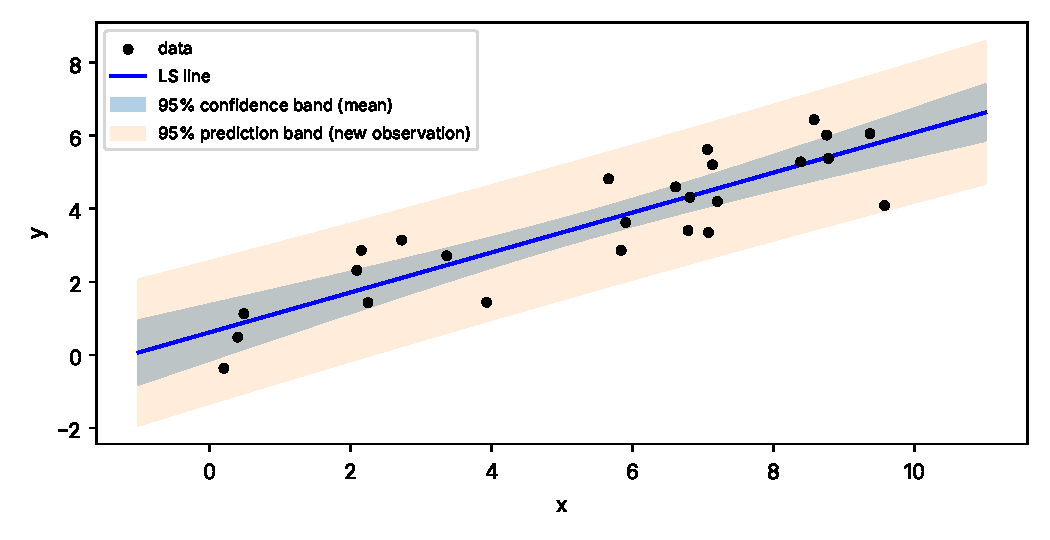
\includegraphics[width=0.8\textwidth]{figures/regresyon_bant.pdf}
\caption{Confidence band (dark) and prediction band (light) in simple regression. The confidence band is narrowest near $\bar x$ and wide at the ends ($q_0$ grows with the distance of $\mathbf x_0$ from $\bar x$); the prediction band is everywhere at least $\pm t\,s$ wide.}
\end{figure}

\section{Comments and Notes}

\begin{remark}[The Hierarchy of Model Assumptions]
It is important to distinguish which assumption an inference relies on:
(i) Unbiasedness requires only $\E\bm\varepsilon=\mathbf 0$ (a correct mean structure).
(ii) The covariance formula $\sigma^2(X^\top X)^{-1}$ and Gauss--Markov\index{gauss markov theorem@Gauss--Markov theorem} additionally require constant variance and uncorrelatedness.
(iii) The exact $t$ and $F$ distributions require normality; however, thanks to Theorem~\ref{thm:ekk-asimptotik}, normality is largely unnecessary in large samples.
The simulation above illustrates this: skewed errors affect the coverage little even for small $n$, whereas heteroscedasticity\index{heteroscedasticity@heteroscedasticity} produces an error that does \emph{not} improve as $n$ grows (the classical coverage stays at $\approx0.93$ even at $n=200$); sandwich\index{sandwich estimator@sandwich estimator} standard errors remove it in large samples. In small samples, however, the sandwich estimator is biased downwards: at $n=10$ its coverage is even lower than that of the classical interval. For small $n$, therefore, the HC3 correction, which uses $e_i^2/(1-h_{ii})^2$ instead of $e_i^2$, is recommended \cite{mackinnon85}.
\end{remark}

\begin{remark}[Advanced Topics]
Natural continuations of this chapter are generalised linear\index{generalised linear model glm@generalised linear model (GLM)} models\index{linear model@linear model} (logistic and Poisson regression\index{poisson regression@Poisson regression}; the likelihood theory is the same as in Chapters~\ref{ch:mle-asimptotik} and~\ref{ch:lrt}), mixed-effects models, regularisation (ridge\index{ridge regression@ridge regression}, lasso) and model selection (AIC, BIC, cross-validation). For the bootstrap in regression see Chapter~\ref{ch:bootstrap}.
\end{remark}

% --- CHAPTER SUMMARY ---
\section{Chapter Summary}
\begin{summary}
\begin{itemize}
  \item The LS estimate solves the normal equations and gives the orthogonal projection of $\mathbf Y$ onto the column space of $X$ (Theorem~\ref{thm:ekk}). The hat matrix $H$ is symmetric and idempotent; its diagonal gives the leverages.
  \item The Gauss--Markov theorem (Theorem~\ref{thm:gauss-markov}): without requiring normality, LS has the smallest variance among linear unbiased estimators (BLUE).
  \item With normal errors $\hat{\bm\beta}$ and SSE are independent (Theorem~\ref{thm:normal-dogrusal}). The $t$ and $F$ tests are exactly valid (Theorem~\ref{thm:f-testi}), and the $F$-test is a likelihood ratio test (Proposition~\ref{prop:f-lrt}).
  \item The prediction interval for a new observation is always wider than the confidence interval for the mean response (Corollary~\ref{cor:regresyon-aralik}).
  \item Without normality, LS is asymptotically normal as the leverages shrink (Theorem~\ref{thm:ekk-asimptotik}). Under heteroscedasticity, sandwich standard errors should be used (Proposition~\ref{prop:sandvic}).
\end{itemize}
\end{summary}
% --- END OF CHAPTER SUMMARY ---

\paragraph{Further reading.} \cite{seber}, \cite[Chapters~11--12]{casella}, \cite[Chapter~13]{wasserman}; for robust standard errors, \cite{white}.

\section{Exercises}

\begin{exercise}\label{exr:17-1}
Show that in simple linear regression $\Cov(\hat\beta_0,\hat\beta_1)=-\sigma^2\bar x/S_{xx}$. What is required of the design for $\hat\beta_0$ and $\hat\beta_1$ to be uncorrelated?
\hfill\hyperref[coz:17-1]{\footnotesize$\rightarrow$\,Solution}
\end{exercise}

\begin{exercise}\label{exr:17-2}
Show that $\sum_ih_{ii}=p$ and $0\le h_{ii}\le1$. The average leverage is $p/n$; write a function that flags high-leverage observations by the rule $h_{ii}>2p/n$. Show that the variance of the residuals is $\Var(e_i)=\sigma^2(1-h_{ii})$; why does this call for ``studentised residuals''?
\hfill\hyperref[coz:17-2]{\footnotesize$\rightarrow$\,Solution}
\end{exercise}

\begin{exercise}\label{exr:17-3}
Compute the bias and covariance of the ridge estimator $\hat{\bm\beta}_\lambda=(X^\top X+\lambda I)^{-1}X^\top\mathbf Y$. Show that for some $\lambda>0$, $\MSE(\hat{\bm\beta}_\lambda)<\MSE(\hat{\bm\beta})$ (total squared loss) \cite{hoerl70}. Does this contradict Gauss--Markov?
\hfill\hyperref[coz:17-3]{\footnotesize$\rightarrow$\,Solution}
\end{exercise}

\begin{exercise}\label{exr:17-4}
For polynomial regression $Y=\beta_0+\beta_1x+\beta_2x^2+\varepsilon$, write code that tests $H_0:\beta_2=0$ with the $F$-test and compares the result with $t^2$. Compute the correlation between $x$ and $x^2$ and the VIF on the interval $x\in[10,11]$; what does centring ($x-\bar x$) change?
\hfill\hyperref[coz:17-4]{\footnotesize$\rightarrow$\,Solution}
\end{exercise}

\end{document}
